\documentclass{article}
\usepackage[utf8]{inputenc}
\usepackage{tikz} %package for plots, graphics and functions

\title{Plotting Curves}
\author{Arman Daneshdoost}
\date{March 2024}

\begin{document}
	\maketitle
	\begin{figure}[h!]
		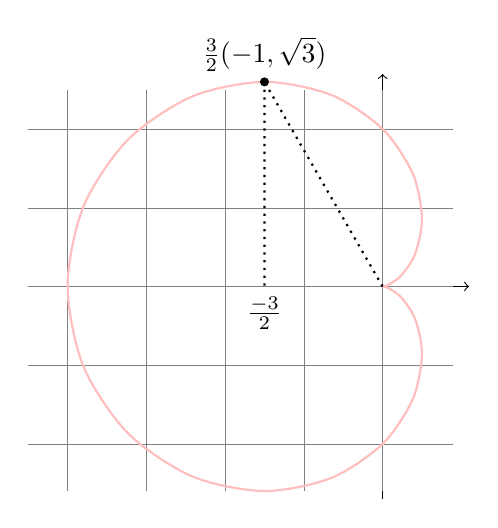
\begin{tikzpicture}
			\draw [ ->] (0, -2.7) -- (0, 2.7);
			\draw [ ->] (-4.5, 0) -- (1.1, 0);
			\draw [gray, ultra thin] (-4.5, -2.6) grid (0.9, 2.5);
			\draw[domain= 0 : 2*pi, smooth, pink, thick] plot ({2*(1-cos(\x r))*cos(\x r)}, {2*(1- cos(\x r))*sin(\x r)});
			% 2pi /3
			\draw[dotted, thick] (0, 0) -- ({2*(1-cos(2*pi/3 r))*cos(2*pi/3 r)}, {2*(1- cos(2*pi/3 r))*sin(2*pi/3 r)})
			node[above] {$\frac{3}{2}(-1, \sqrt{3})$};
			\draw [fill] ({2*(1-cos(2*pi/3 r))*cos(2*pi/3 r)}, {2*(1- cos(2*pi/3 r))*sin(2*pi/3 r)}) circle [radius = 0.05];
			\draw[dotted, thick] ({2*(1-cos(2*pi/3 r))*cos(2*pi/3 r)}, {2*(1- cos(2*pi/3 r))*sin(2*pi/3 r)}) -- (-3/2, 0) node [below] 
			{$\frac{-3}{2}$};
		\end{tikzpicture}
	\end{figure}
\end{document}